\noindent{\sffamily\small\bfseries\color{C3}PART I · WORKFLOW CONSTRUCTION}
\section{从既有分工到连续执行}
\subsection{继承共同基础，不重新编造起点}
上一份已验收Process Report已经记录了我与GPT、Codex之间的分工、双报告、来源审核、证据与远程审查方式。本次沿用这套共同基础，不把实验一的算法、参数、结果和截图当成新实验材料。报告视觉继续使用P2，科研图保留原生可编辑源；工作流和体系图提供draw.io及SVG/PDF。

我提供的本轮执行提示词把总体方案标为已确认，并要求“先保证正确，再追求优秀；先做基础实验，再研究组合”。这是当前可访问的执行授权依据，早先网页讨论的未提供原文没有被重新编写。研究目标、教师要求和关键评价不能由执行器随意改变，但范围内的普通参数、调试、控制变量和已有父项支持的组合可以连续执行，避免每一步都退回让我确认同一件事。

\subsection{真正变化的是反馈和恢复责任}
这次的难点不止是填完TODO。教师材料把在线尾部体验、静态Pareto前沿与动态长期收入放在一起，既有算法语义冲突，也有数据分区和成本遗漏风险。我要求Codex先建立可信基线，再根据实际结果决定下一轮；普通缺陷必须修复、回归、重建受影响产物，然后回到未完成的父任务。合法方法没有收益时则保留负结果，不把它强行修成正结果。

执行上因此形成两条不同回路。工程回路处理实现或评价偏离：复现问题、固定新版本、使旧结果失效并重跑。研究回路处理效果和机制：读数、假设、单因素、父项、必要组合、取舍。前者的修复次数不是后者的效果提升次数。这一区分在KM指标、Double随机流和主动调度中都实际发挥了作用。

\section{真实独立上下文怎样参与}
\subsection{六类职责，四个实际上下文}
本轮确实启用了原生子Agent，而不是给函数换名字。主线程承担协调、基础在线实现与文稿集成；research\_data负责材料、来源和数据，随后独立核验进化分支；evolution负责多目标实现与实验，随后独立核验RL；reinforcement负责RL和加分机制，随后独立核验在线匹配和交付边界。研究、设计、执行、核验、批判和制图六类职责按先后交接分配给四个实际上下文。

各角色能读写同一工作区，但任务合同限制可改对象：原始资料和批准合同保持只读，模块分工明确。重要交接包含输入版本、问题、允许方法、结果路径、验证方式及返回条件。对自己算法的检查只记作者自检，交叉核验者必须重新取原始输入和实际产物。

\begin{figure}[htbp]\centering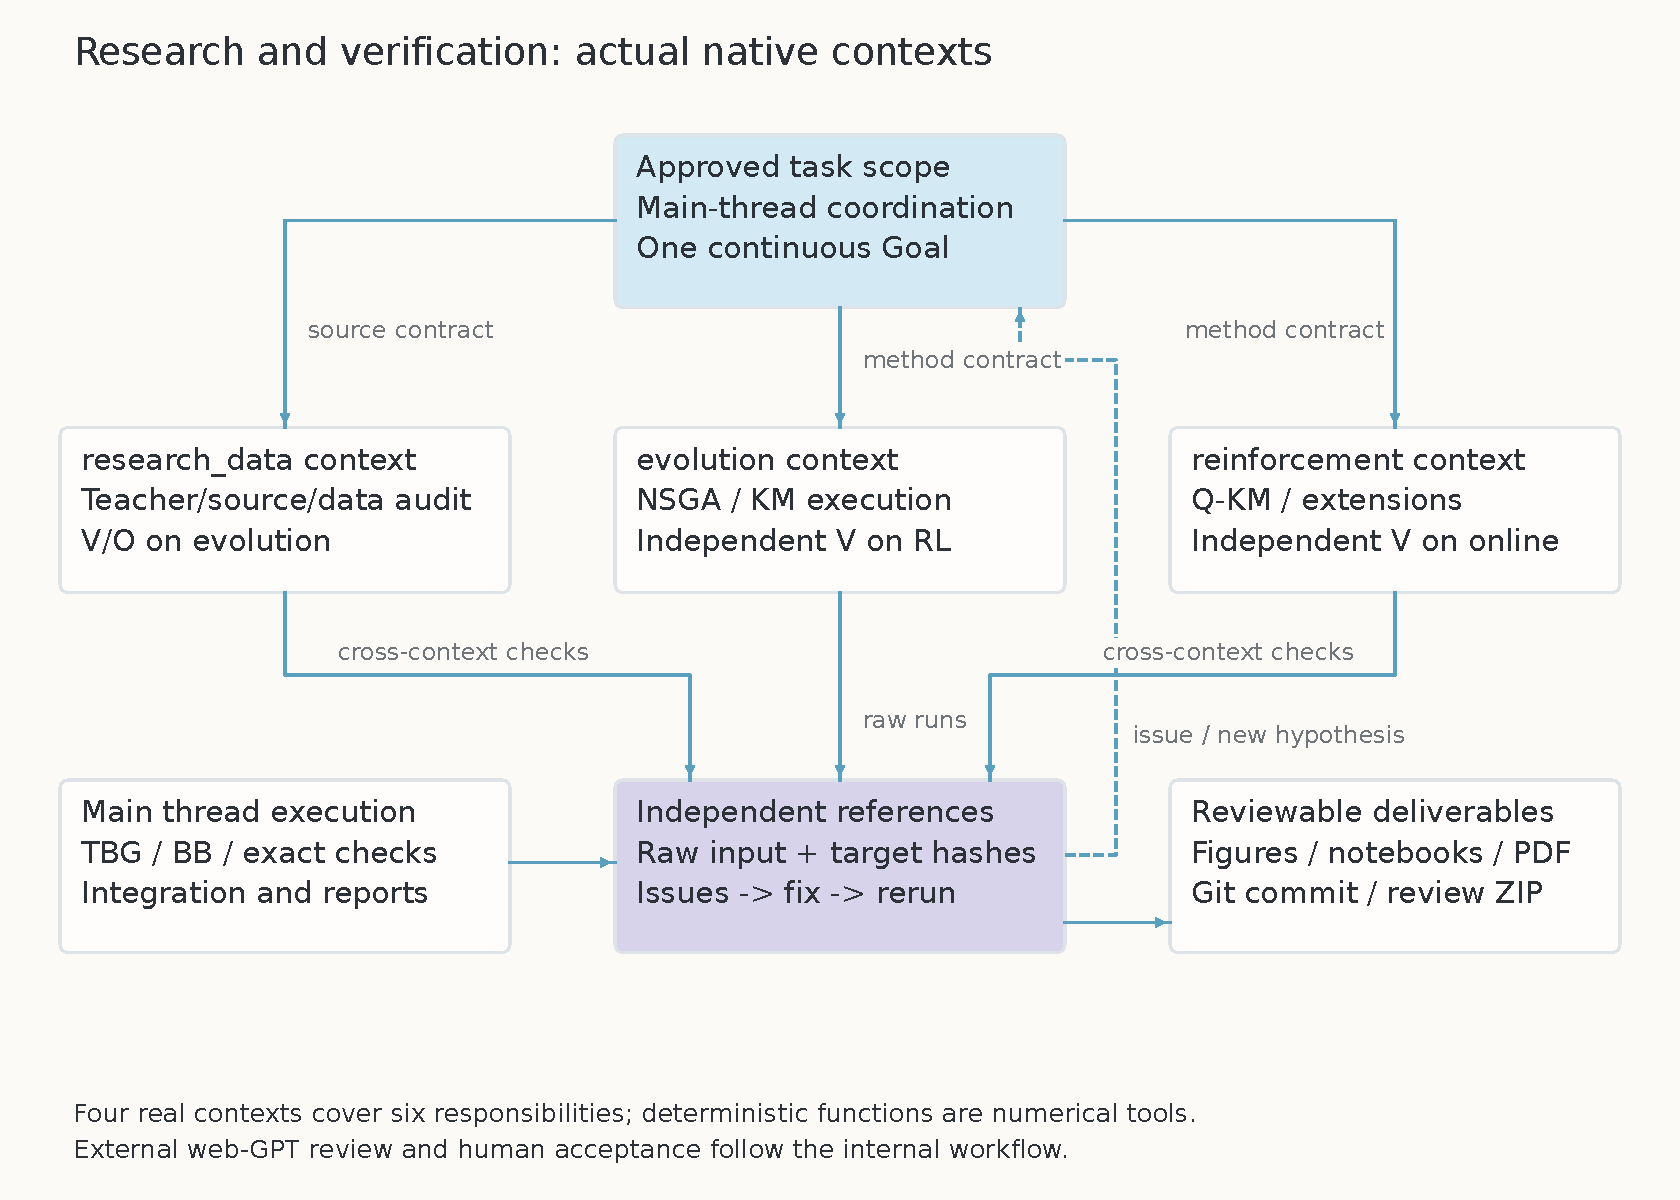
\includegraphics[width=\linewidth]{../../diagrams/research_verification_workflow.pdf}
\caption{本次真实研究与独立核验职责。四个原生上下文分时承担六类职责；箭头表示任务合同、产物和问题反馈。图解释实际技术组织，不替代原始对话UI证据。}\label{fig:processworkflow}\end{figure}

\subsection{反馈并非执行者自己的PASS}
在线分支的核验者从输入与匹配记录重新算距离、等待、唯一性和离线目标，并另写小图参考。进化核验者从原批次重解码基因，再独立求目标与HV；他发现Spacing包含了不应进入前沿的点，并提前发现初始化成本不在计时内。RL核验者没有调用作者仿真器，而是按原订单和trace重建忙闲、移动和取消，再核对Double公式和动态NSGA选点。

这些角色返回的是可定位的问题和独立读数，主线程继续落实修复，而不是收到一份审查报告就结束整个任务。没有调用付费模型API或远程GPU，也没有把最终确定性派单声称为每单一次LLM通信。原生独立上下文的真实协作与课程模型中的司机决策是两个层次。
